\chapter*{Введение. Обоснование актуальности} % * не проставляет номер
\addcontentsline{toc}{chapter}{ВВЕДЕНИЕ} % вносим в содержание

Компьютерная графика, как часть компьютерных наук, существует уже более 70-ти лет и на данный момент содержит в себе множество различных алгоритмов, позволяющих получать фотореалистичные изображения в режиме реального времени. Однако, несмотря долгую историю, большая часть упомянутых алгоритмов применима только для симуляции и отображения объектов, представляемых как наборы абсолютно твердых тел. 

Относительно недавно, был разработан метод PBD\cite{pbd}, позволяющий симулировать взаимодействие мягких тел. Данный метод быстро стал стандартом для симуляции таких объектов как ткани, жидкости, подушки и т.д. Хочется отметить, что данный метод обильно применяется для представления различных органов в системах для подготовке к хирургическим операциям \cite{li2022position}. Вскоре, данный метод PBD получил множество улучшений, главным из которых можно выделить появление метода XPBD\cite{xpbd}, позволяющего использовать табличные физические величины реального мира для задания параметров симуляции мягких тел.

Однако на практике, даже у тел симулируемых методом XPBD, может наблюдаться неестественное поведение, отличающееся от поведения наблюдаемого в реальном мире. Зачастую, описанное поведение представляет собой периодичные перемещения с большой амплитудой различных частей симулируемого тела (\firef{fig:streching}), и может достигаться как резким и сильным взаимодействием с телом (например резко подул сильный ветер). Для того, чтобы бороться с такими ситуациями в рамках метода XPBD существует два решения. Первое - поставить условия симуляции таким образом, чтобы подобных взаимодействий не возникало, однако это не всегда возможно. Второе - указывать более высокую точность, что будет требовать больше вычислений и неприемлемо в условиях симуляций реального времени. 

\begin{figure}[ht!] 
	\center
	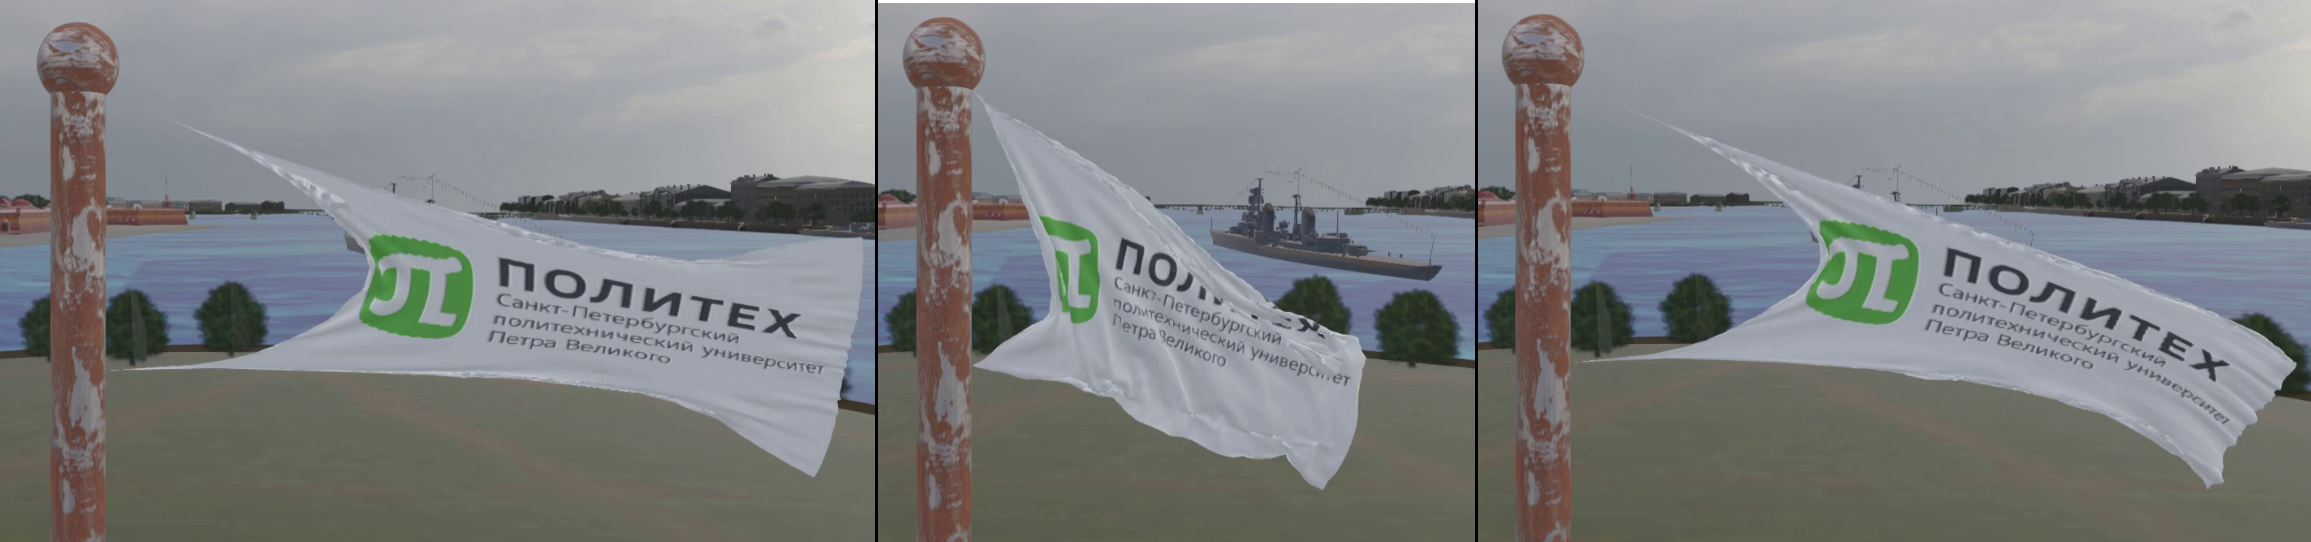
\includegraphics [scale=0.25] {my_folder/images//streching}
	\caption{Пример неестественного растяжения в результате сильного ветра.\newline Кадры сняты спустя 1, 2 и 3 секунды после запуска симуляции.}
	\label{fig:streching}  
\end{figure}

В рамках данной работы, была поставлена цель разработать и реализовать эмперический алгоритм, позволяющий бороться с вышеописанной ситуацией, при этом не требуя много больше процессорного времени. Помимо этого была поставлена цель реализации метода XPBD с использованием GPU, и последующее сравнение реализованных алгоритмов с реализацией из библиотеки NVidia Cloth.


%Данный пример выпускной квалификационной работы (далее --- ВКР) создан для того, чтобы продемонстрировать возможности шаблонов SPbPU-student-templates, выполненных с помощью издательской системы \LaTeX{} \cite{spbpu-student-thesis-template}. В примере отображены некоторые обязательные элементы ВКР \cite{spbpu-student-thesis-specification}. Для того, чтобы подробнее ознакомиться с требованиями к наполнению этих элементов, а также с общими требованиями к структуре и оформлению ВКР, пожалуйста, ознакомьтесь с  \cite{spbpu-student-thesis-template-author-guide,spbpu-student-thesis-specification}. 

%Пример может быть использован для подготовки отчета по практике с учетом корректировки требований к титульному листу, структуре и содержанию конкретной практики в соответствии с планом её проведения (рабочей программы дисциплины).


%Технология написания ВКР на \LaTeX{} подробно изложена в \cite{spbpu-student-thesis-template-author-guide}. В рекомендациях приведены ссылки на учебно-справочные материалы \LaTeX{} (под \LaTeX{} в документе может подразумеваться также \TeX, \LaTeXe).


%Авторам, использующим \LaTeX{}, необходимо последовательно заменять текст данного шаблона в файлах <<\verb|thesis.tex|>> на текст своей ВКР, избегая при этом ошибок (errors) при компиляции. Синтаксические конструкции \LaTeX, которые задействованы в формировании того или иного текста выделены \texttt{машинописным шрифтом}. Иные шрифты в тексте ВКР (за исключением математических) использовать запрещено. 

%Светлым курсивом выделены \textit{важные} элементы текста (ключевые слова определений, интонационные выделения словосочетаний), полужирным шрифтом --- \textbf{служебные} элементы текста (<<определение>>, <<теорема>>, <<лемма>> и т.п), а также при необходимости ключевые слова в алгоритмах. В соотношении к основному тексту курсив и полужирный шрифт не может превышать 1 \% текста на странице.
 
%Полужирный курсив разрешено использовать только в \textbf{\textit{названиях подпараграфов (пунктов)}} и запрещёно использовать в основном тексте. 
%\uline{Подчеркивание} допускается использовать только в задании в местах, где данные вписываются студентом, а также в математических формулах при необходимости.

%Введение \textit{не должно превышать 4 страницы}. Во введении необходимо обосновать выбор темы, охарактеризовать современное состояние изучаемой проблемы, ее актуальность, практическую и теоретическую значимость, степень разработанности данной проблемы.


%\textbf{Aктуальность исследования} заключается в N фактах и явлениях,  а также в их состоянии, связанных с ними нерешенных проблемах, слабо освещенных и требующих уточнения или дальнейшей разработки вопросов. 

%\textbf{Объект исследования} --- это то, на что направлен процесс познания (индивид, коллектив, общность людей, сфера деятельности и т.п.). Связь объекта и предмета легко запоминаются по формуле: <<исследуем такой-то объект на предмет чего-то>>. Это процесс или явление, порождающее проблемную ситуацию, и избран-ное для изучения в целом. Всегда в объекте содержится предмет, а не наоборот. 

%\textbf{Предмет исследования} --- один из аспектов, часть рассматриваемого объекта (свой-ства, состояния, процессы, направления и особенности деятельности структур по связям с общественностью, их сотрудников в конкретных сферах общественных отношений и т.д.). Предмет исследования частично совпадает с названием работы и содержится в цели сразу после сказуемого (<<выявить \ldots что?>>, <<определить \ldots что?>>, <<сформировать \ldots что?>>). Именно предмет исследования определяет тему выпускной квалификационной работы.
%Объект и предмет исследования соотносятся между собой как целое и частное, общее и частности. 


%\textit{Цель исследования} формулируется, исходя из проблемы, которую следует разрешить студенту в процессе выполнения выпускной квалификационной работы и представляет собой в самом сжатом виде тот результат (результаты), который должен быть получен в итоге исследования. Формулировку цели рекомендуется начинать со слов: <<сформировать/создать>>, <<разработать>>, <<провести>>, <<подготовить>>.

%\textbf{Цель исследования} --- краткий ожидаемый результат, то есть решение практических задач и новые знания о рассматриваемом предмете исследования. 
%В соответствии с целью исследования, логически определяются следующие \textbf{задачи работы} (должно быть \textit{не менее четырех задач, но не более шести задач}):

%\begin{enumerate}
%	\item Первая задача.
%	\item Вторая задача.
%	\item Третья задача.
%	\item Четвертая задача.
%\end{enumerate} 


%Задачи отражают \textit{поэтапное достижение цели, при этом уточняют границы проводимого исследования}.
%Рекомендуется формулировать задачи с глаголов в форме перечисления: <<изучить \ldots>>, <<выявить \ldots>>, <<проанализировать \ldots>>, <<разработать \ldots>>, <<описать \ldots>> и т.п. Заголовки выпускной квалификационной работы должны отражать суть поставленной задачи.


%Общая направленность исследования задается до его начала сформулированными \textbf{гипотезами}, которыми могут быть:
%\begin{itemize}
%	\item научное предположение, выдвигаемое для объяснения каких-либо факторов, явлений и процессов, которые надо подтвердить или опровергнуть (т. е. требующее верификации);
%	\item вероятностное знание, научно обоснованная догадка по объяснению действительности;
%	\item прогноз ожидаемого решения проблемы, ответ на вопрос, поставленный в задаче;
%	\item условно-категорическое умозаключение по схеме <<если \ldots, то \ldots>>, основными элементами которого являются условие (причина) и результат (следствие).
%\end{itemize}  

%Гипотеза --- это предполагаемое решение проблемы. В ходе исследования гипотезу проверяют и либо подтверждают, либо опровергают. Формулировка гипотезы \textit{обязательна только для магистров}.


%\textbf{Теоретическая и методологическая база исследования}. В теоретической базе необходимо перечислить источники, которые использовались для написания работы. Приведём примеры ключевых фраз: 
%\begin{itemize}
%	\item <<Теоретической основой выпускной квалификационной работы послужили исследования  \ldots (перечисляются конкретные документы)>>.
%	\item <<Практическая часть работы выполнялась на основании документов  \ldots>>.
%	\item  <<При написании выпускной квалификационной работы использовалась работы отечественных и зарубежных специалистов \ldots>>.
%	\item  <<Для выполнения анализа в практической части были использованы материалы  \ldots>>.
%	\item <<При подготовке ВКР были использованы материалы таких учебных дисциплин, как "Технология конструкционных материалов'', "Экономика'' "Начертательная геометрия'' \ldots>>.
%	\item <<При выполнении ВКР использовались материалы N организации \ldots (ссылка на официальный сайт)>>.
%\end{itemize}

%\textbf{Методологическая база исследования} должна содержать указание на методы и подходы, на которых основывается данная ВКР. 

%Среди методов исследования студенту необходимо обратить внимание на общенаучные методы, включающие эмпирические (наблюдение, эксперимент, сравнение, описание, измерение), теоретические (формализация, аксиоматический, гипотетико-дедуктивный, восхождение от абстрактного к конкретному) и общелогические (анализ, абстрагирование, обобщение, идеализация, индукция, аналогия, моделирование и др.) методы.
%Также следует назвать конкретно-научные (частные) методы научного познания, представляющие собой специфические методы конкретных наук: экономики, социологии, психологии, истории, логики и проч.

%\textbf{Информационной базой} для разработки ВКР служат материалы, собранные студентом в процессе обучения в ВУЗе, в ходе прохождения учебной и производственной практик, а также во время прохождения преддипломной практики.
%Дополнительная информационная база может включать информацию официальных статистических публикаций (например, Госкомстата России), материалы, получаемые из Интернета, информацию международных организаций и ассоциаций. 

%\textbf{Степень научной разработанности проблемы} --- это состояние теоретической разработанности проблемы, анализ работ отечественных и зарубежных авторов, исследующих эту проблему. Здесь важно подчеркнуть исторические, экономические, политические или профессиональные явления, повлиявшие на выбор темы. Также в данной части введения проводится критический обзор современного состояния и освещения исследуемой темы в научной, профессиональной литературе и СМИ, обобщаются и оцениваются точки зрения различных авторов по теме исследования. 

%\textbf{Научная новизна} выявляется в результате анализа литературных источников, уточнения концептуальных положений, обобщения опыта решения подобных проблем. Это принципиально новое знание, полученное в науке в ходе проведенного исследования (теоретические положения, впервые сформулированные и обоснованные, собственные методические рекомендации, которые можно использовать в практике).
%Научная новизна выпускной квалификационной работы может состоять: 
%\begin{itemize}
%	\item в изучении фактов и явлений с помощью специальных научных методов и междисциплинарных подходов;
 %   \item в изучении уже известного в науке явления на новом экспериментальном материале;
%	\item в переходе от качественного описания известных в науке фактов к их точно определяемой количественной характеристике;
%	\item в изучении известных в науке явлений и процессов более совершенными методами;
%	\item в сопоставлении, сравнительном анализе протекания процессов и явлений;
%	\item в изменении условий протекания изучаемых процессов;
%	\item в уточнении категориального аппарата дисциплины, определение типологии, признаков, специфики изучаемого явления.
%\end{itemize}

%\textbf{Практическая значимость} подробно отражается в:
%\begin{itemize}
%	\item практических рекомендациях или разработанном автором выпускной квалификационной работы проекте (как основная часть выпускной квалификационной работы);
%	\item выявлении важности решения избранной проблемы для будущей деятельности магистра по выбранному направлению подготовки.
%\end{itemize} 

%Практическая значимость выпускной квалификационной работы может заключаться в возможности:

%\begin{itemize}
%	\item решения той или иной практической задачи в сфере профессиональной деятельности;
%	\item проведения дальнейших научных исследований по теме ВКР;
%	\item разработки конкретного проекта, направленного на интенсификацию работы исследуемой организации, предприятия.
%\end{itemize}

%\textbf{Апробация результатов} исследования включает:
%\begin{itemize}
%	\item участие в конференции, семинарах и т. д.;
%	\item публикации по теме выпускной квалификационной работы;
%	\item применение результатов исследования в практической области;
%	\item разработку и внедрение конкретного проекта;
%	\item выступления на научных конференциях, симпозиумах, форумах и т.п. (\textit{обязательно});
%	\item публикации студента, включенные в список использованных источников. 
%\end{itemize}


%В силу ограниченности объема необходимо очень тщательно подойти к написанию введения, которое должно стать <<визитной карточкой>>, кратко, но емко характеризующей работу. Во введение не включают схемы, таблицы, описания, рекомендации и т.п. 

%Целью первой главы, как правило, является всесторонний анализ предмета и объекта исследования, второй --- разработка предложений (алгоритмов, технологий и т.п.) по улучшению какого-либо процесса, протекающих с участием предмета и объекта исследования, третьей --- практическая реализация (имплементация) --- предложений (алгоритмов, технологий и т.п.) в виде программного (или иного) продукта, четвертой --- апробация разработанных в работе предложений и выводы целесообразности их дальнейшей разработки (использованию). 
%Содержание глав в данном шаблоне приведено только для демонстрации возможностей \LaTeX.


%% Вспомогательные команды - Additional commands
%\newpage % принудительное начало с новой страницы, использовать только в конце раздела
%\clearpage % осуществляется пакетом <<placeins>> в пределах секций
%\newpage\leavevmode\thispagestyle{empty}\newpage % 100 % начало новой строки